\chapter{Desenvolvimento do projeto}
\label{chap:metod}
 Nesta seção, serão apresentados os métodos e processos utilizados para o desenvolvimento do portfólio digital, incluindo a metodologia adotada, a arquitetura geral do sistema, os requisitos técnicos e a modelagem dos processos. O objetivo é fornecer uma visão clara e estruturada das etapas envolvidas na criação do portfólio, desde a concepção até a implementação.

\subsection{Metodologia do projeto}
    A metodologia adotada para o desenvolvimento deste portfólio digital é baseada no modelo ágil, que prioriza a flexibilidade, a colaboração e a entrega incremental de valor. O processo foi dividido em etapas, começando com o levantamento de requisitos, seguido pela modelagem do sistema, prototipagem e testes. Essa abordagem permite uma adaptação rápida às mudanças nas necessidades do cliente e garante que o produto final atenda às expectativas.

\subsubsection{Gerenciamento Ágil de Projetos}
O gerenciamento ágil, inspirado no framework Scrum~ \cite{schwaber2001agile}, orientou o andamento do projeto. A plataforma Trello foi utilizada para acompanhamento das atividades em sprints quinzenais.

\subsubsection{Engenharia de Requisitos}

 De acordo com Sommerville~\cite{kotonya1998requirements}, a engenharia de requisitos é uma etapa fundamental no desenvolvimento de software, pois envolve a identificação, análise e documentação das necessidades do cliente. No caso deste portfólio digital, foram realizadas reuniões com o cliente para entender suas expectativas e requisitos funcionais e não funcionais. A partir dessas informações, foi possível elaborar um documento de requisitos que serviu como base para as etapas seguintes do projeto.

\section{Ideação}
%escrever oq sera apresentado

A fase de ideação foi crucial para o desenvolvimento do portfólio digital, onde foram levantadas as necessidades e expectativas do cliente. A equipe realizou reuniões com o cliente para entender suas demandas, preferências estéticas e funcionais, além de analisar portfólios digitais similares no mercado. Essa etapa inicial permitiu a definição clara dos objetivos do projeto e a identificação dos requisitos essenciais.

\subsection{Arquitetura Geral}
 A estrutura da arquitetura do portfólio digital foi concebida para ser intuitiva e responsiva, garantindo uma experiência de usuário fluida em diferentes dispositivos. A camada de apresentação é responsável pela interface do usuário. Dando a ela um design responsivo, utilizando HTML e CSS para a estrutura e estilo, respectivamente. O JavaScript foi integrado para adicionar interatividade e dinamismo à interface como algumas animações.

\begin{figure}[H]
    \centering
    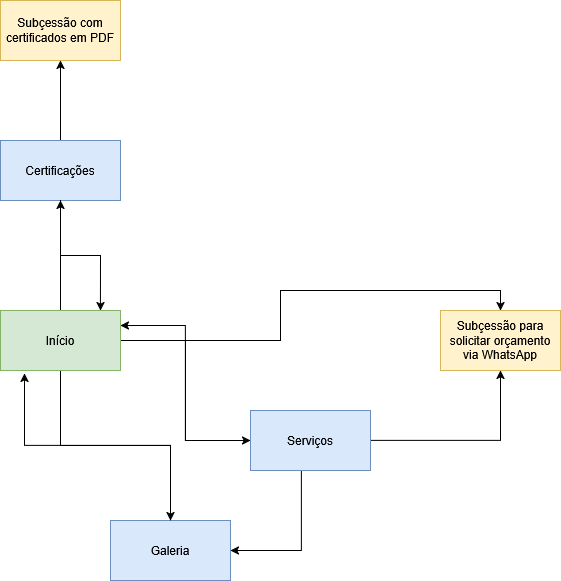
\includegraphics[width=0.6\textwidth]{Figures/arquitetura.png} % use your image path and name here
    \caption{Arquitetura.}
    \label{fig:Arquitetura}
\end{figure}

Neste conjunto se encontram as páginas principais do portfólio, como a página inicial, a seção de projetos e a página de contato.

\subsection{Requisitos técnicos}

Os requisitos técnicos foram definidos com base nas necessidades do cliente e nas melhores práticas de desenvolvimento web. A seguir, estão os principais requisitos:
\begin{itemize}
    \item \textbf{Tecnologias Utilizadas:} HTML, CSS e JavaScript.
    \item \textbf{Funcionalidades:} O portfólio deve incluir uma página inicial, uma seção de projetos, uma página de contato e uma seção de certificados.
    \item \textbf{Responsividade:} O design deve ser responsivo, adaptando-se a diferentes tamanhos de tela, incluindo dispositivos móveis e desktops.
    \item \textbf{Desempenho:} O site deve carregar rapidamente e ser otimizado para uma boa performance, mesmo em conexões lentas.
    \item \textbf{Manutenção:} O código deve ser bem documentado e organizado, facilitando futuras manutenções e atualizações.
\end{itemize}

%desdobramento da função qualidade
\subsection{Quality Function Deployment}

O QFD (Quality Function Deployment) foi utilizado para garantir que as necessidades do cliente fossem traduzidas em requisitos técnicos claros e mensuráveis. Através de uma matriz QFD, foram identificadas as prioridades do cliente e como elas se relacionam com as características do sistema. Essa abordagem ajudou a alinhar as expectativas do cliente com as funcionalidades do portfólio digital.

 \begin{figure} [H]	
     \centering
     \caption{ Primeiro ciclo QFD}
     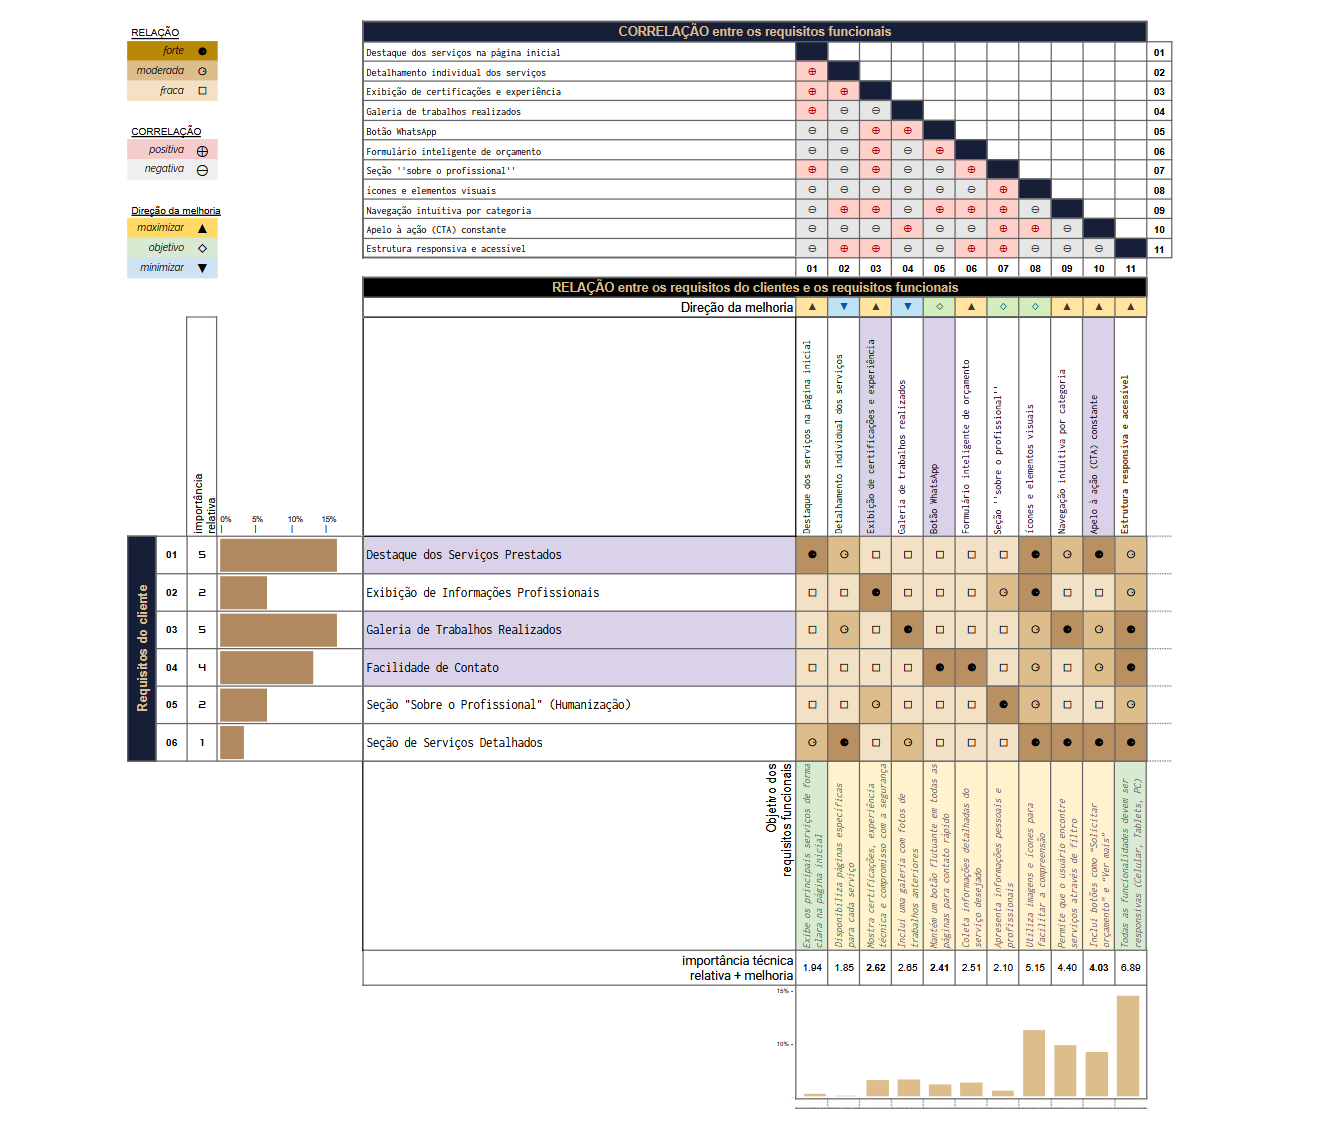
\includegraphics[width=0.8\textwidth]{Figures/matrizqfd.png}
     \caption*{Matriz-QFD}
     \label{fig:QFD}
\end{figure}
   

% % %--------- NEW SECTION ----------------------
% % \section{Interface do Usuário}
% % \label{sec:ui}
% % \lipsum[1]

% % %--------- NEW SECTION ----------------------
% % \section{Simulação do sistema}
% % \label{sec:sim}
% % \lipsum[2-4]
\subsection{Modelagem dos processos}

 O BPMN (Business Process Model and Notation) foi utilizado para modelar os processos envolvidos no desenvolvimento do portfólio digital. Essa abordagem permitiu uma visualização clara dos fluxos de trabalho, facilitando a identificação de etapas críticas e a otimização dos processos. A modelagem BPMN também ajudou a garantir que todos os membros da equipe estivessem alinhados quanto às responsabilidades e prazos.


Essas informações advieram do modelo esquematico de processos, no qual consultamos o cliente para entender suas necessidades e expectativas.

\begin{figure}[H]
    \centering
    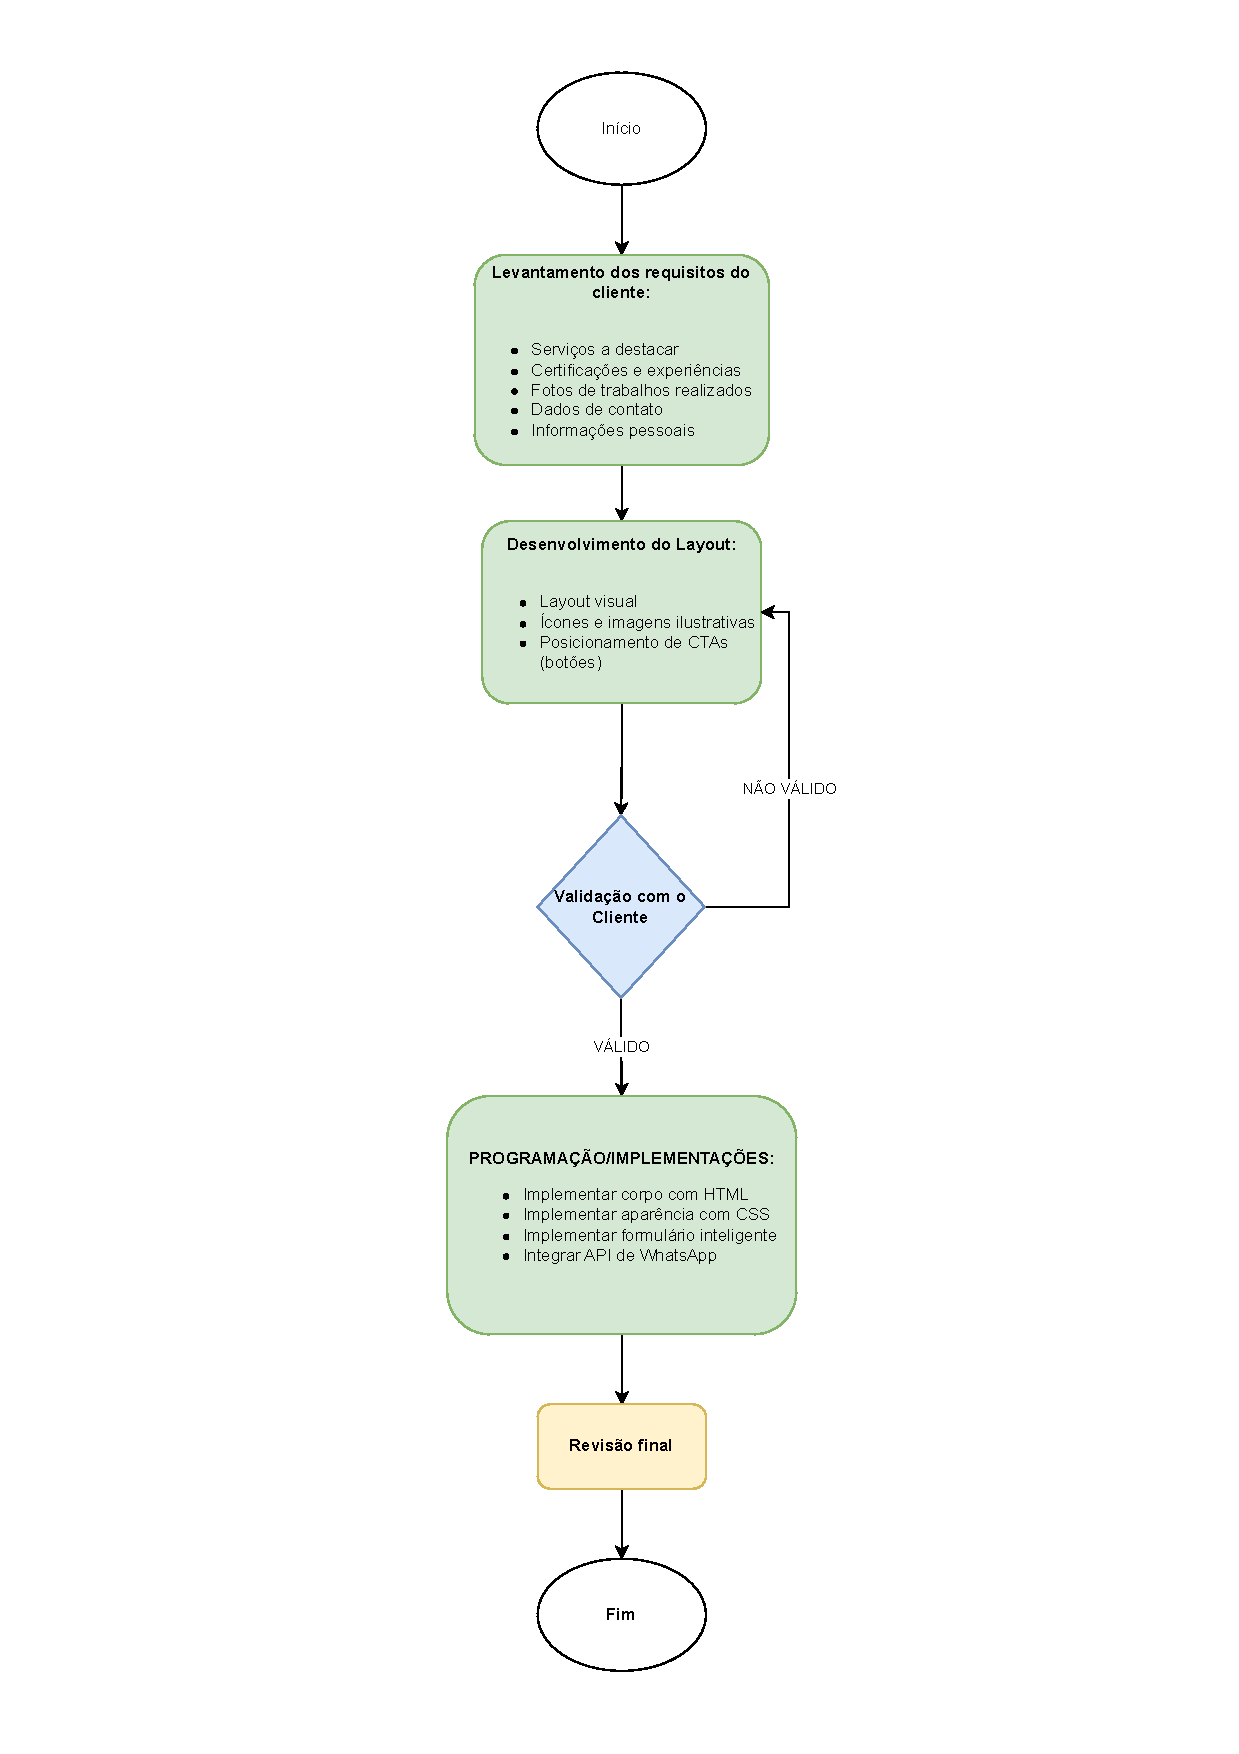
\includegraphics[width=0.6\textwidth]{Figures/modelo_esquematico_de_processos..pdf} % use your image path and name here
    \caption{Modelo esquemático de processos.}
    \label{fig:esquema}
\end{figure}




